\documentclass[12pt]{article}
\renewcommand{\familydefault}{\sfdefault}
\usepackage[a4paper, margin=1in]{geometry}
\usepackage{graphicx}

% Title Page
\title{Data analysis work-flow for morphological profiling}
\author{Sundaramurthy Lab}

\begin{document}
\maketitle



\section{Biological motivations}
We at the bug lab in NCBS are interested in understanding host pathogen interactions and developing new tools to understand the fundamentals. We are a group of 13 people working on different projects. 
\begin{enumerate}
	\item The projects are broadly divided into 3 categories. First being the malaria group that aims to develop the in vitro liver stage model of plasmodium infection to further the understanding of plasmodium pathogenesis and have an assay for the drug screening.
	People are also involved in understanding the role of hepatic polarity in the pathogenesis of the parasite. 
	\item Another group of people are working to understand the tuberculosis pathogenesis and its exploitation of the host trafficking pathways of endocytosis and autophagy. They induce and track the pathways and notice how infection has changed, and vice versa. 
	\item And there is another group of people who do quantitative image analysis optimizing segmentation, writing macros for 3D segmentation, developing new data analysis techniques and presenting new ways to look at the data.
\end{enumerate}

	\begin{center} 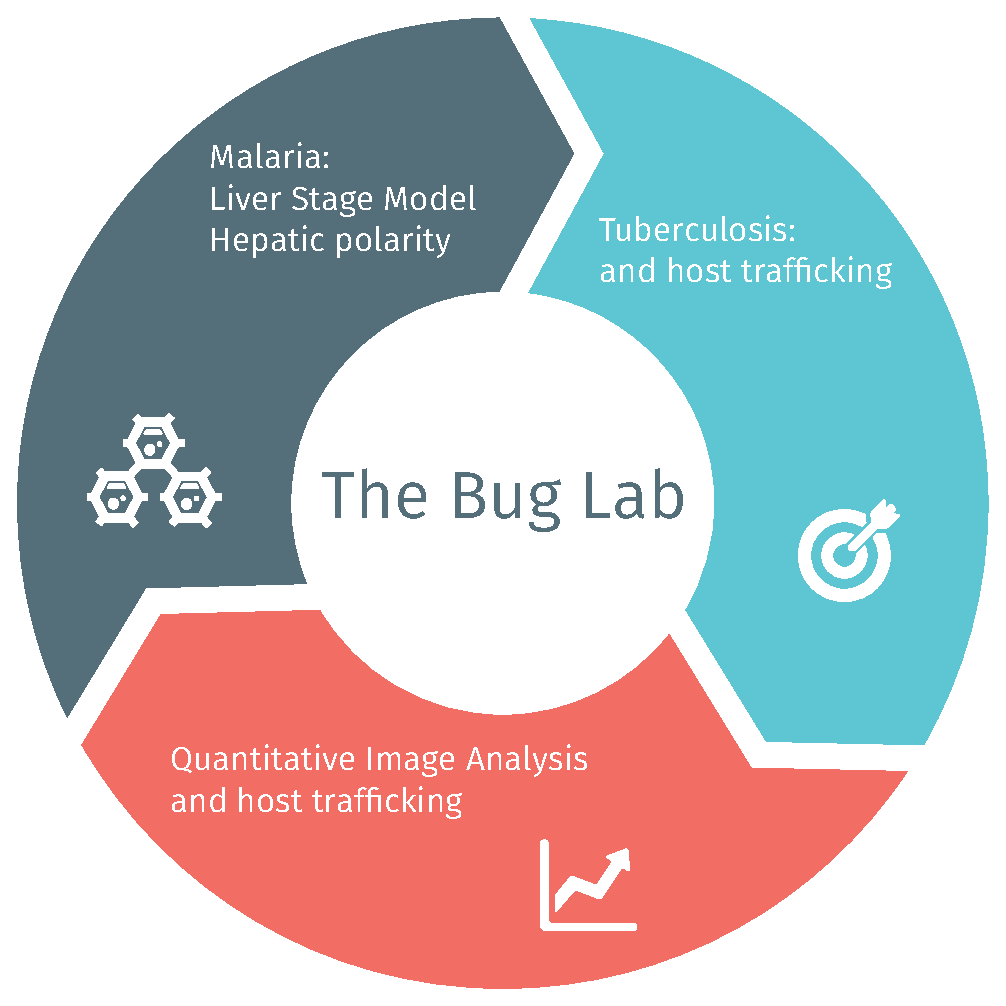
\includegraphics[width=4in]{svg/Lab_Interests.eps} \end{center}

In our lab we use widefield, confocal, and EM microscopies. The images can be single slice images, Z-stacks, and high throughput. For image processing CellProfiler is the most common software but MotionTracking, FIJI are also regularly used. For data analysis we primarily use R and KNIME. 


\section{Image analysis and feature extraction}
The primary software used for image analysis and segmentation of the fluorescent microscopy images is CellProfiler. 

\begin{center} 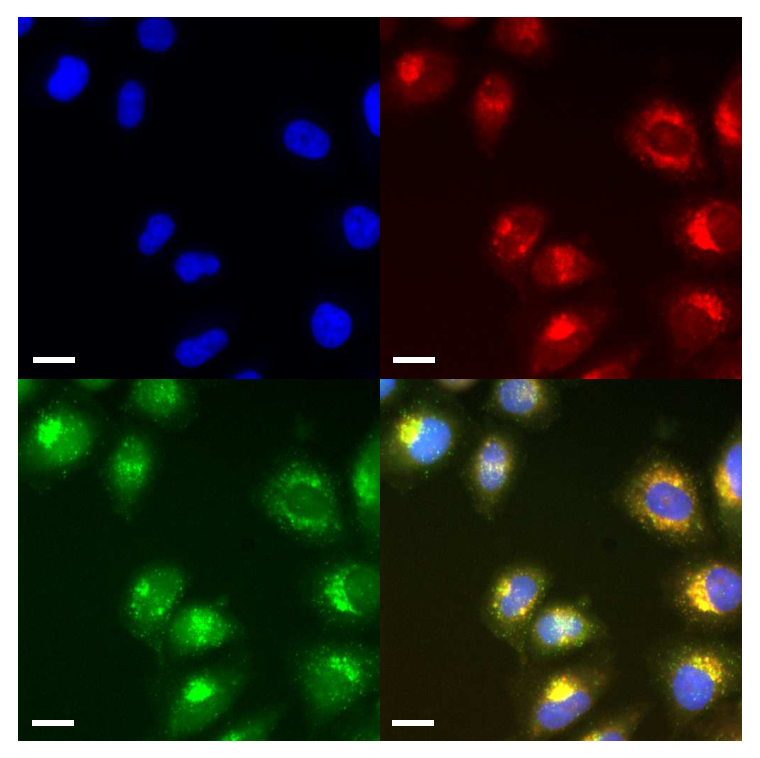
\includegraphics[width=5in]{svg/drawing.eps} \end{center}

The image analysis pipeline typically involves the following steps:
\begin{enumerate}
	\item Rescaling Intensities
	\item Illumination Correction: Calculate and Apply
	\item Enhance/ Suppress features for easier segmentation of the small puncta
	\item Identification of primary object (typically nucleus), secondary object (typically cell), other cellular organs (like endosomes, autophagosomes, lysosomes, infectious agents, etc.)
	\item Identify colocalization of different objects
	\item Relate objects
	\item Measure features (Area/Shape, intensities, spatial spread, etc) of the objects identified. Also calculate per cell mean values for all the object features
	\item Export the images of objects identified
	\item Export the measurements
\end{enumerate}
MotionTracking, that is built on Pluk platform (http://pluk.mpi-cbg.de/projects/motiontracking), is also regularly used. FIJI is used for 3D segmentation.


\section{Image quality control}
	\begin{enumerate}
	\item Flag images based on focus score to remove out of focus images
	\item Plot plate maps to see if the plate variability exists
	\end{enumerate}
	

\section{Data cleaning}
	\begin{enumerate}
		\item Experiments conducted at different times can have novel nomenclature used (like dapi, DAPI, Dapi; identify these differences and replace with consistent nomenclature)
		\item Different image analysis software will result in their own nomenclature of the feature names, like in MotionTracking the feature names have special symbols like $! . = ( ), etc$ which are not handled well by R. So those column names are renamed to get rid of special symbols
		\item Sometimes additional metadata features have to be added to the data files like the infection status in the infection study that is added based on the bacterial count. Also if binning analysis has to be done, the new Metadata\_Bin column is created at this stage
		\item There are lot of NAs in the data. We need to get rid of them
			\subitem Get rid of those columns which contain just NA
			\subitem Get rid of those rows with more than some percentage of NAs, lets say $~ 50\%$. This is uncommon.
			\subitem There are some NAs that are converted to 0 (like bacterial features in non-infected cells)
		\item Features with 0 standard deviation are removed
	\end{enumerate}


\section{Data filtering}
\begin{enumerate}
	\item There are apoptotic cells/ improperly segmented cells (that are detected based on cell area/ eccentricity (artifacts)), 
	\item Number of nuclei/cell must be 1.
	\item Then we check that the cell filtering has removed roughly equal amounts of cells from each treatment conditions, else there might be an inherent bias in that well, which might or might not be a phenotype, and will need further scrutiny. 
\end{enumerate}
	\begin{center} 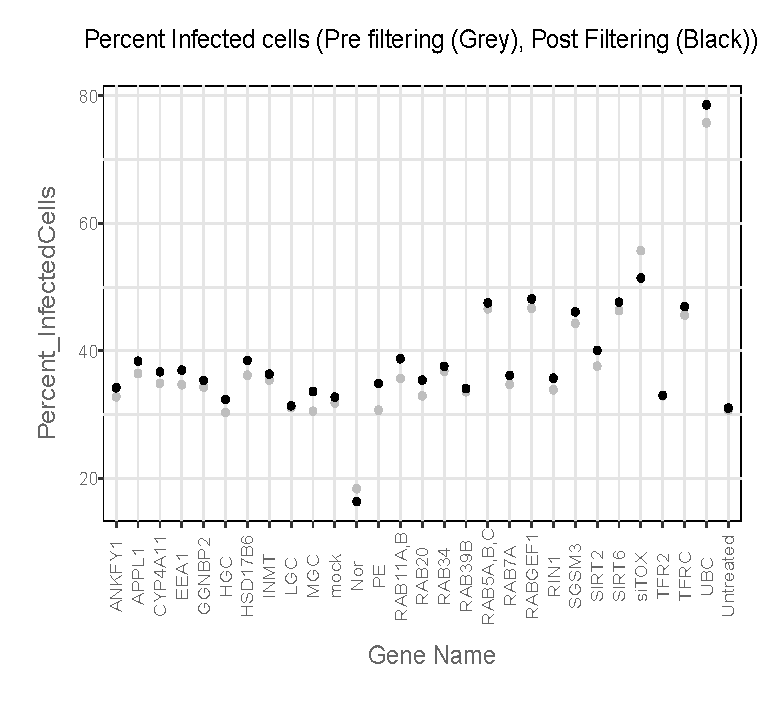
\includegraphics[width=5in]{svg/Filtering.eps} \end{center}
	

\section{Normalize features}
Normalization is important if we are to compare the strength of phenotype in different features, and also across assays.
	\begin{enumerate}
		\item Robust Normalization with the formula\\
		$z\hbox{-score}_{\rm NC} = \frac{Value - Median [Values_{\rm NC}]}{MAD_{\rm NC}}$ \\
		is done typically. It is more resistant to outliers.
		\item Classical Z-scoring is required in conditions when the robust normalization results in NAs (which regularly happen in the conditions where median value of a feature is zero, like bacterial counts). In those times we resort to the following formula\\
		$z\hbox{-score}_{\rm NC} = \frac{Value - Mean [Values_{\rm NC}]}{\sigma_{\rm NC}}$ \\
	\end{enumerate}
	The per treatments Zscore is shown in this plot and we can see that we get z-scores of  > 2 in case of the Positive controls, and multiple negative controls occur in the narrow range. 
	\begin{center} 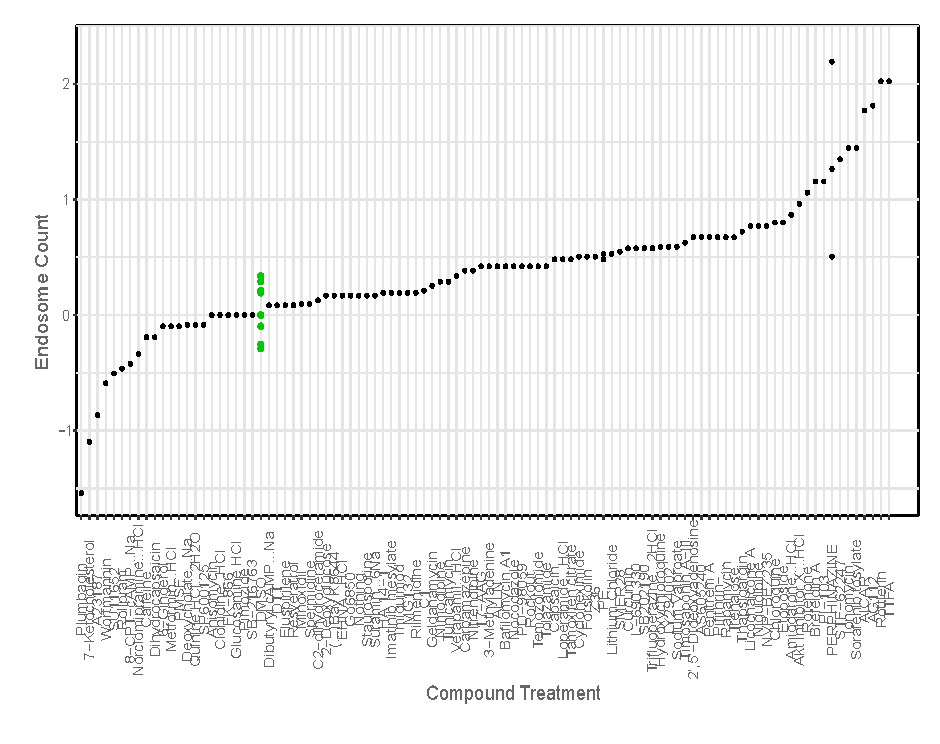
\includegraphics[width=6in]{svg/S1_shared_zscores_2_1.eps} \end{center}
	

\section{Transform features}
The feature Transformations like principle component analysis and factor analysis have been tried and did not yield favorable results. \\
The normalization is also a type of feature transformation that is regularly employed. It is easy to make out the differences in different treatment conditions after transforming the data to Z-scores. \\
The density plots of all observations are made to identify the parent distribution. If the distribution is flat for some features, those features are removed from subsequent analysis, these features introduce significant noise when feature reduction techniques like PCA are applied. Also these features can not be removed using the redundant feature removal.


\section{Correct for systematic effects}
	When ever a high throughput experiment is conducted, there are redundant conditions typically negative controls that are spread all across the plate in both horizontal and vertical direction that is used to access if there are any systemic plate bias. 
	Plot plate layouts for different known features and visualize the well variability in the plate, if high throughput. We have rarely found a systemic bias in plates. 
	\begin{center} 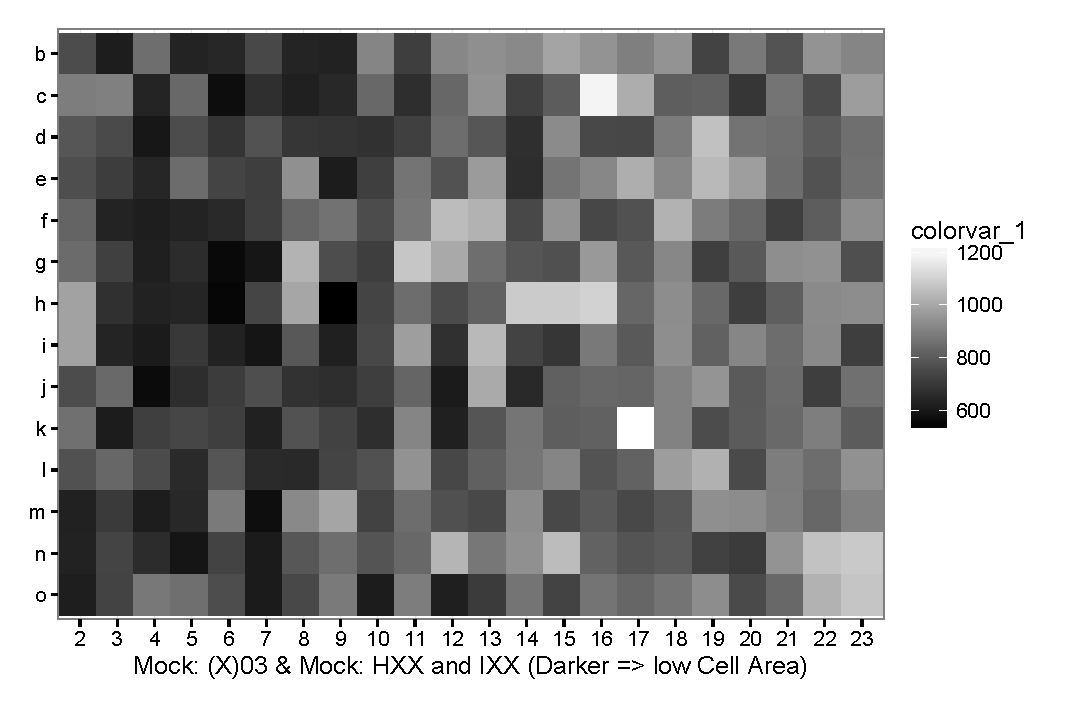
\includegraphics[width=6in]{svg/plate_layout_cell_area.eps} \end{center}	
	

\section{Select features}
	\begin{enumerate}
		\item The features are selected based on non-redundancy. Only one feature out of the set of features with redundancy more than 0.90 (pearson correlation coefficient) is selected. The feature that minimizes redundancy with every other feature with correlation coefficient less than 0.90 is selected from a set of redundant features.
		\item The features are tagged as those belonging to either of the two categories, metadata space and features space. So that vectorized mathematical operations can be performed on the feature space while grouping the data based on one or multiple metadata columns.
		\item Since we have to regularly deal with different plates with different readouts in the same experiment, we mark the common features as "shared features" and others as "unshared features". Shared features are compared across different plates, and compared for reproducibility. If reproducibility is confirmed, then the unshared features can be compared. These comparisons are typically visualized in the form of boxplCots.
	\end{enumerate}
	

\section{Create per-well profiles}
	\begin{enumerate}
		\item The individual sub-cellular object is collapsed to per cell values by taking median or sum as appropriate (for instance, median in case of MeanIntensity, sum in case of IntegralIntensity)
		\item Next the per-cell values are calculated by taking the median of all the values in a specific condition. If the data set has multiple redundant conditions like different siRNAs, then they are collapsed per siRNA treatment and accessed for per siRNA changes in phenotypes.
		\item If a metadata column for binning analysis was made, then the collapsing is done using median value per bin per condition.
	\end{enumerate}
	

\section{Measure similarity between profiles}
	\begin{enumerate}
		\item The magnitude of phenotype is visualized in box plots, and density plots (or heat maps if conditions to be analyzed are a lot).
		\begin{center} 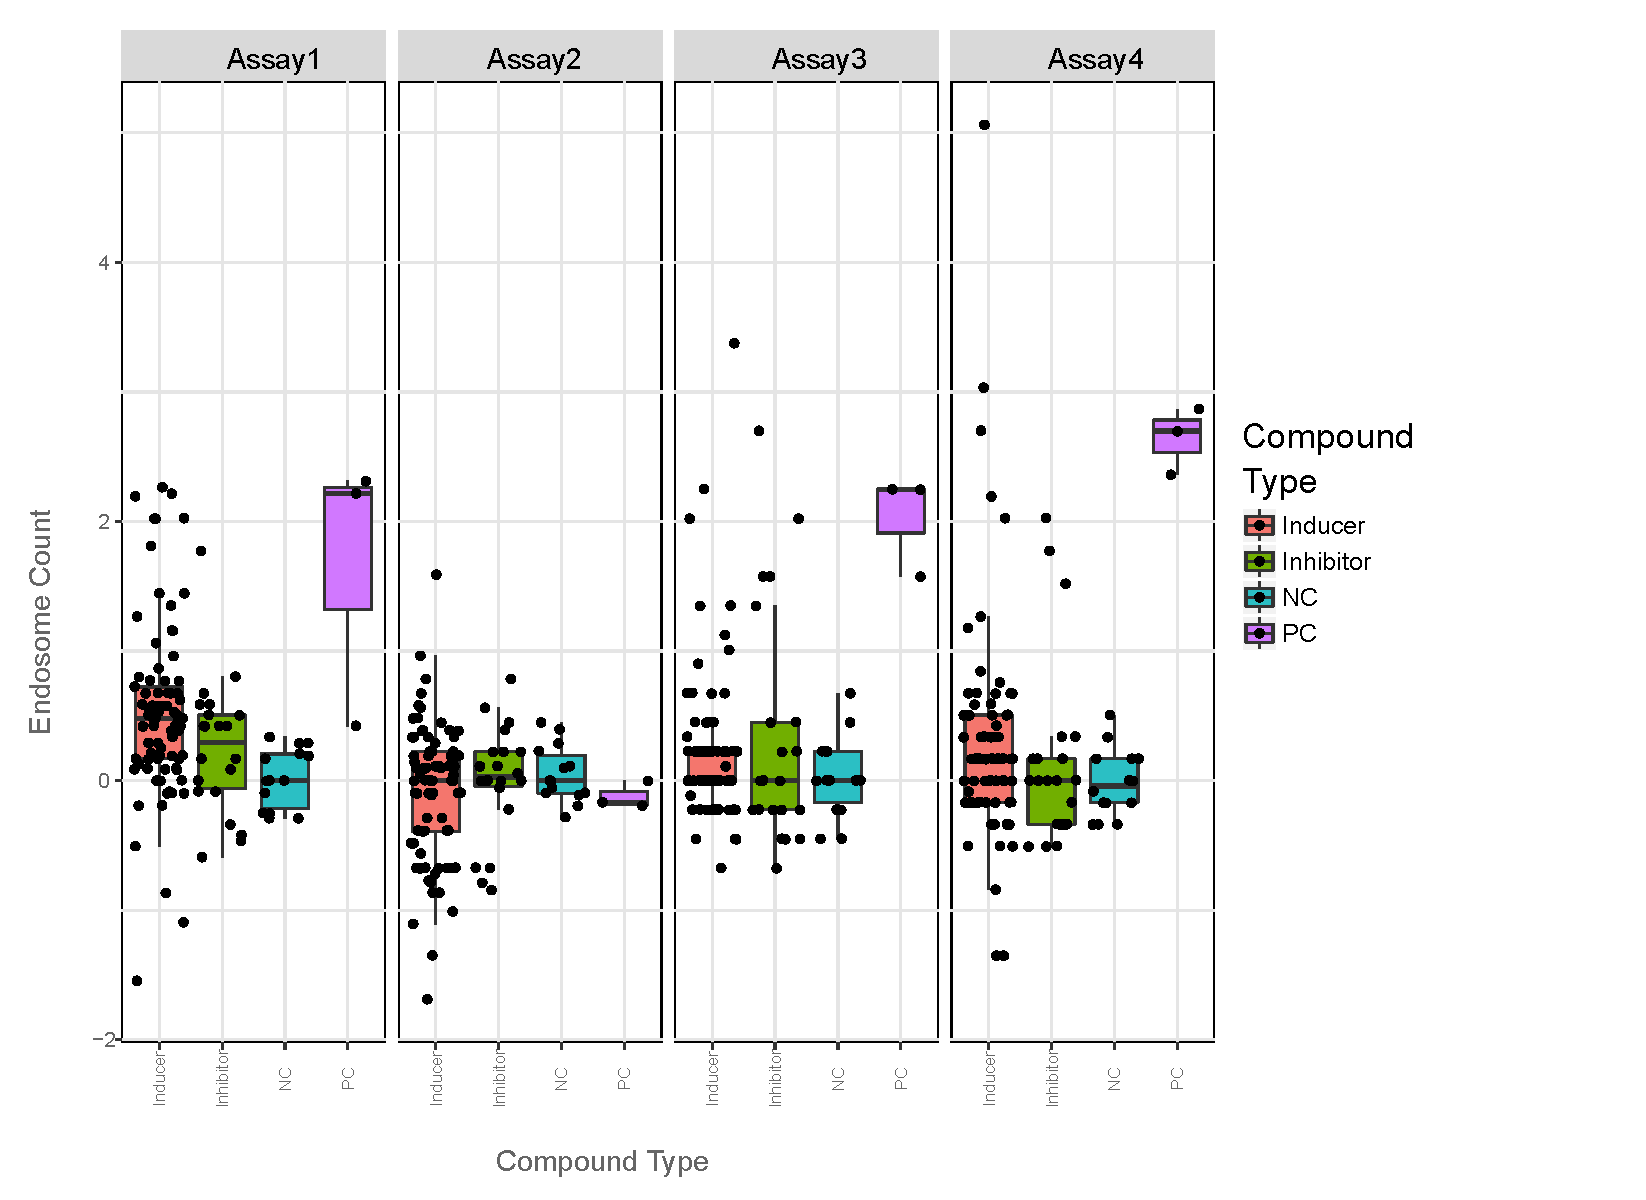
\includegraphics[width=6.5in]{svg/S1_unshared_boxplot_2.eps} \end{center}	
		\item Similarity between profiles is measured using Pearson correlation coefficient
		\item The quantitative significance between different conditions and control is done by tests of significance (mostly students T test, and Kolmogorov-Smirnov test). This step puts number to the significance that we already see in the box plots. Inferences of an increase or decrease are made from the box plots plotted previously.
		\item Another way to assess the similarity between different phenotypes is hierarchical clustering, that clusters the phenotypes based in similarity amongst themselves, one instance is shown in the following cluster dendrogram.
		\begin{center} 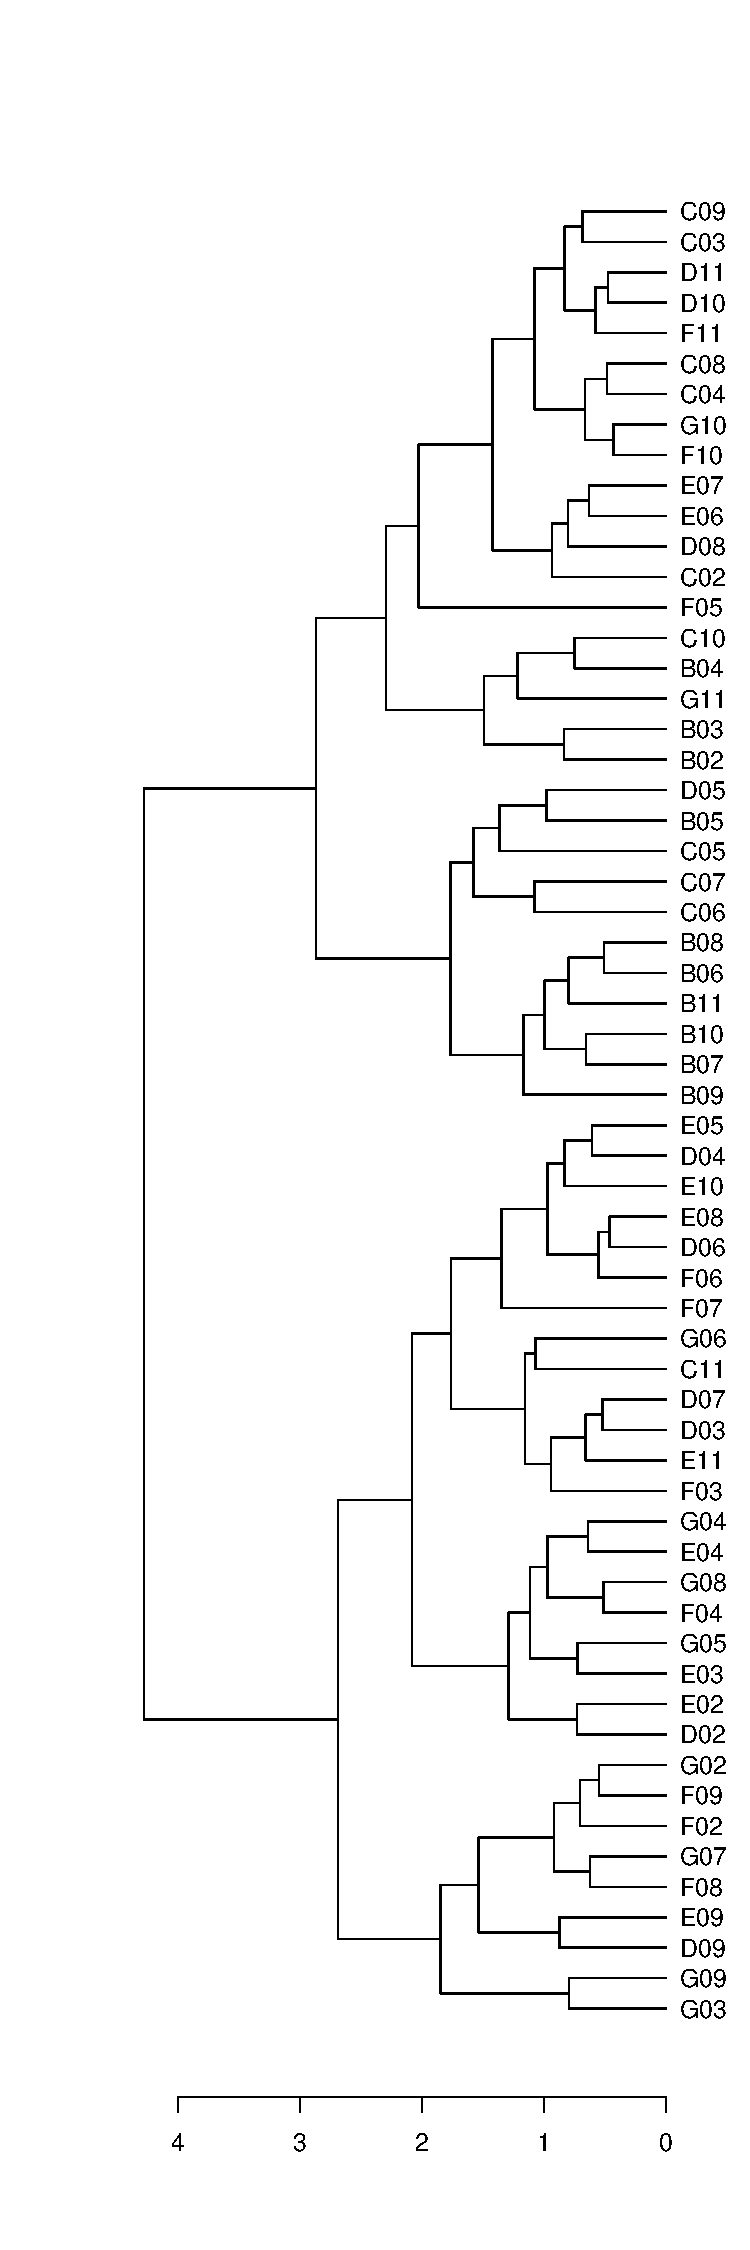
\includegraphics[width=2.1in]{svg/dendo.pdf} \end{center}	
	\end{enumerate}
	

\section{Integrate different plates}
Spectral limitations allow for only few channels to be visualized at a time in the biological sample, greatly limiting simultaneous visualization of the different sub-cellular organelles. In order to overcome this problem at the post-imaging stage, data from different plates/ assay but that are a part of same experiment need to be plotted in one plot.\\
In our lab, permutation testing is being tried to integrate the data from different assays. We define the null  and alternate distribution based on the similarity matrix between the reps and non-reps (by reps we mean the correlation coefficient of the same treatments across different plates and by non-rep we mean the different treatments in the same/different plates). Once the significance of phenotype is established, then exact p-value is calculated as shown in the plot. 
	\begin{center} 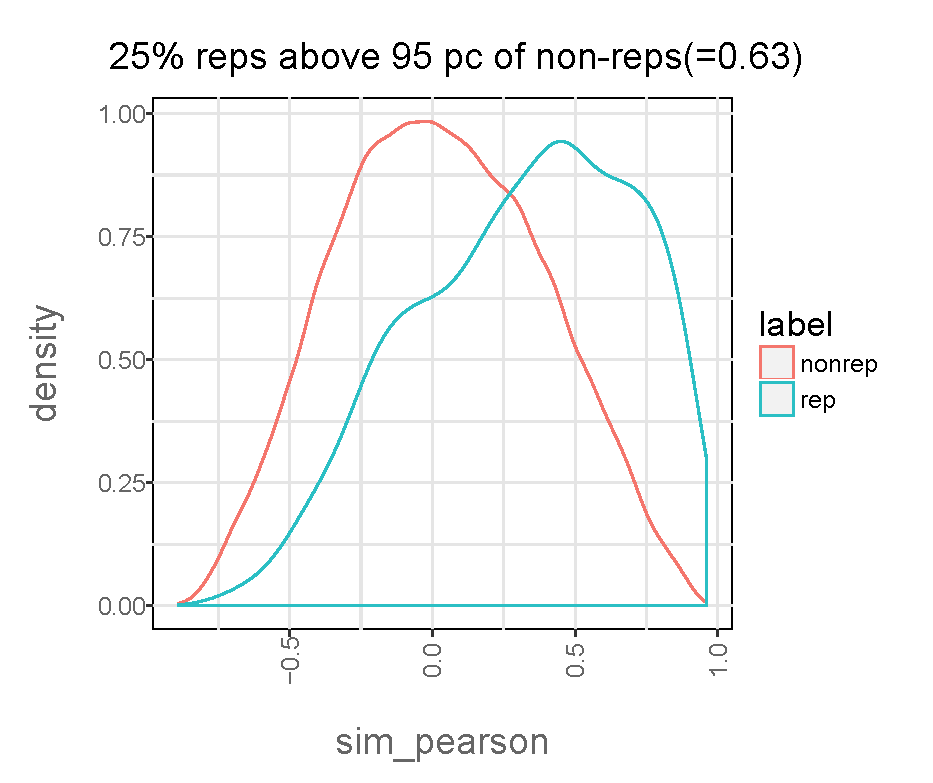
\includegraphics[width=4in]{svg/S1_rep_non_rep.eps} \end{center}	
This p-value for different pair of assays is amenable for comparison and is plotted on the scatter plot. This plot explains when the two pairs of assays are behaving in same way, in other words, if same treatment results in similar changes in two different cellular organelles. 
	\begin{center} 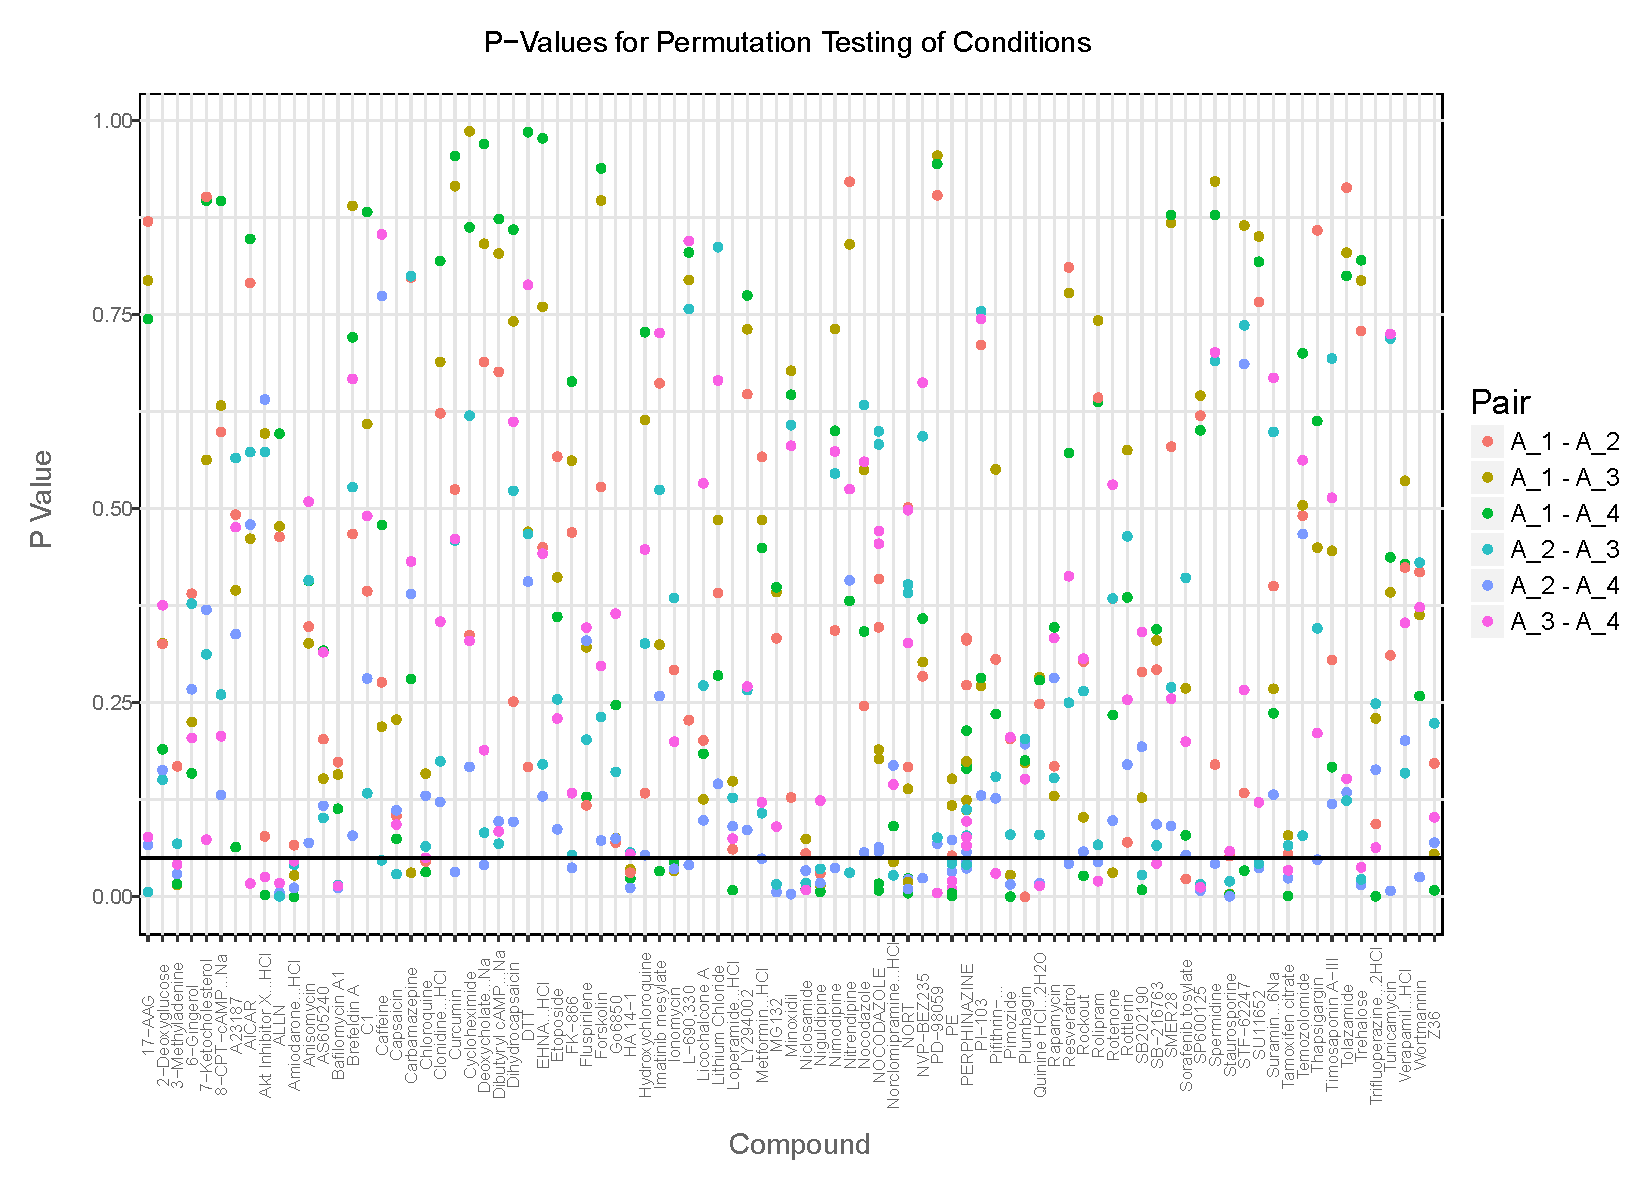
\includegraphics[width=6in]{svg/S1_p_value_unshared_filtered_signifiant.eps} \end{center}	



\end{document}          



Hi Shantanu, 
I have arrived in Boston (right now in north quincy with family). Let meet up tomorrow. Could you let me know whats your contact number.
See you tomorrow.
Harmanjit Singh
1 (646) 417-0372
